\section{Aufbau des Systems}
\subsection{Systembeschreibung}
% Bild für Systembeschreibung
\begin{figure}[htbp]
\centering 
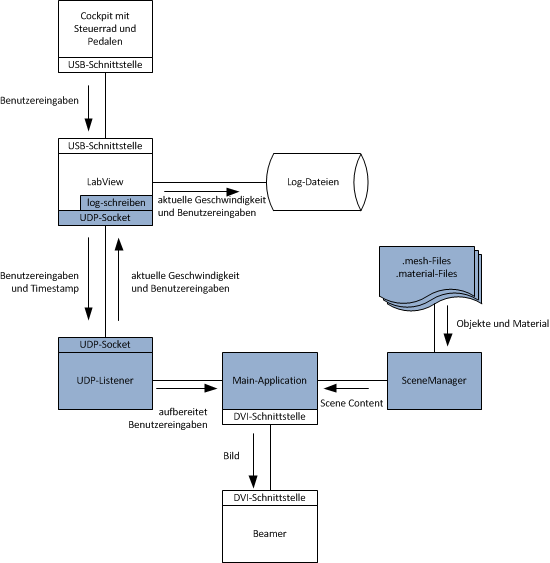
\includegraphics{src/Systembeschreibung.png}
\caption{Systembeschreibung} % Titel der Grafik
\label{Systembeschreibung} % Labelname
\end{figure}

Der Aufbau des Systems für den Fahrsimulator haben wir uns wie in Abbildung \ref{Systembeschreibung} überlegt. Die Komponenten die blau markiert sind, müssen von uns entwickelt werden, die anderen bestehen bereits. 
Die Benutzereingaben die im Cockpit gemacht werden, werden bereits von einem LabView Programm eingelesen. Es benötigt lediglich noch einen UDP-Port über den wir die verschiedenen Eingaben an unser Programm weiterleiten können. Zusätzlich wird der UDP-Port auch für das empfangen verschiedener Log-Daten, die von unserem Programm gesendet werden, verwendet. Zu diesem Zweck muss das Lab-View Programm ebenfalls erweitert werden, damit die Empfangenen Daten sauber in ein Log-File geschrieben werden. 
Nun muss in C einen UDP-Socket mit entsprechendem UDP-Listener implementieren werden um die Benutzereingaben zu erhalten. Der UDP-Listener wird gleichzeitig verwendet um Geschwindigkeit des Fahrzeugs sowie Timestamp und weitere Daten an das Lab-View zurück zu schicken, damit diese gespeichert und später Ausgewertet werden können. Diese Aufteilung durch eine Netzwerkschnittstelle, ermöglicht es uns unser System, wenn notwendig, zu dezentralisieren. Dies wird im Ralisierungskapitel des UDP-Listeners genauer ausgeführt. In einem ersten Schritt wurde der UDP-Listener in einem Video-Beispiel, nachzulesen im Anhang A, implementiert und getestet. 
Die Position des Steuerrades und der Gas und Brems-Pedalen werden vom UDP-Listener permanent das Hauptprogramm übergeben. Dieses wertet die Positionen aus und veranlasst die entsprechenden Aktionen in der geladenen Scene. 
Die Scene selbst wird von einem Scenen-Manager geladen. Dieser benötig für die zu ladenden Objekte die Definition der Objekte in der Form eines mesh-Files und mindestens ein Materialfile in dem die benötigten Texturen und Materialien definiert sind. Die berechnete Scene wird in einem Fenster von Hauptprogramm angezeigt und über eine DVI-Schnittstelle an den Beamer übertragen. Der Beamer projeziert das Bild an die Wand die sich direkt vor dem Cockpit befindet. 

\subsection{Anforderungen}
\subsubsection{Funktionelle Anforderungen}

\subsubsection {Nicht Funktionale Anforderungen}
\renewcommand{\labelenumi}{\alph{enumi})}
\begin{enumerate}
\item Zuverlässigkeit
\item Benutzbarkeit
\item Aussehen und Handhabung
\item Wartbarkeit
\item Zeitliche Anforderungen
\end{enumerate}
